\documentclass[12pt]{article}
\usepackage{tikz}
\usetikzlibrary{shapes,snakes}
\usepackage{algorithm}
\usepackage{algorithmic}%\usepackage[pagebackref=true,colorlinks,linkcolor=blue,citecolor=magenta]{hyperref}
\usepackage{graphicx} 
\usepackage{fancybox}
\usepackage{setspace}  
\usepackage[colorlinks,linkcolor=blue,citecolor=magenta]{hyperref}
\usepackage{enumerate} 
\usepackage{amsthm,amssymb,amsmath}
\usepackage{indentfirst}
\usepackage{listings}
\usepackage{mathtools}
\newtheorem{theorem}{Theorem}
\newtheorem{lemma}{Lemma}
\newtheorem{definition}{Definition}
\usetikzlibrary{fit}

\begin{document}

\title{Draft of Hypertree Decomposition}
\date{\today}
\maketitle
\section{Introduction}
In this draft we will talk about the hypertree decomposition and effect of using it on delta queries computations. The main contribution of this paper is that it proves that the total number of nodes in all hypertree decomposition of all delta queries is polynomial.
\section{Preliminaries}
Throughout this paper, for the sake of simplicity, we are dealing only with Boolean Conjunctive Query (BCQ) and we call them query. These results can be extended to other queries as well. Suppose we are given a query and we want to evaluate it. This is called \emph{evaluation problem} and is an NP-complete problem\cite{1}. Thus, generally it is not solvable with a polynomial algorithm, but in some restricted versions we can solve this problem in polynomial time. \par

One important class for which we have polynomial algorithms is \emph{Acyclic Queries}. 

We use $var(Q)$ to show the set of variables in query $Q$ and $relations(Q)$ denotes the set of relations in query $Q$.
\begin{definition}
\label{def:primalgraph}
The primal graph of query $Q$ is a graph $G(V,E)$. where $V=vars(Q)$ and for all relations $A$ and for all $a,b\in vars(A)$ we add an edge between $a$ and $b$. $E=\{(a,b)|\exists A: a\in vars(A)\land b\in vars(A)\}$
\end{definition}
\begin{definition}
\label{def:hypergraph} 
The hyper graph of query $Q$ is a hyper graph $G(V,E)$ where $V=var(Q)$ and for each relation $A$ we add an hyper edge among all $var(A)$.
\end{definition}
When the primal graph of a query is acyclic then we can call it the \emph{Join Tree}. As previously stated we can evaluate a query in polynomial time when we have its join tree. Although we rarely encounter acyclic queries, in many cases we can decompose the primal graph into a tree. For example we can use a tree decomposition algorithm on the primal graph to obtain a tree. After decomposing the query, some nodes will have more than one relation, thus, the maximum number of relations in any node is called tree width. 
Decomposing a graph into a tree is an NP-Complete problem, but if we know the tree width is constant, then there is a polynomial time algorithm for that. \par
%Bounded treewidth is very common for queries, we can guess an upper bound on the treewidth and then compute the tree decomposition. 
\begin{definition}
\label{def:dualgraph}
The dual graph of query $Q$ is a graph $G(V,E)$. where $V=relations(Q)$ and for each relation $A$ for which we have $var(A)\cap var(B)\neq \emptyset$, we add an edge between $A$ and $B$. $E=\{(a,b)|var(a)\cap var(b)\neq\emptyset\}$
\end{definition}
The definition of dual graphs~\eqref{def:dualgraph} came from the dual of hypergraph. 
\subsection{Generalization for inequalities and nested queries}
\label{sec:generalization}
In the previous section we have presented the notions of graph and hyper graph models for queries which only contain equal joins. In those models we can not have any inequalities or any nested queries. But in this section we want to generalize those models for these two case. We consider each inequalities as an imaginary relation between two variables. Imaginary here means that we don't need to materialize it. Thus, in hyper graph representation each inequality $a\theta b$ is a hyper edge on $a$ and $b$. In dual graph modelling it is a vertex which is connected to other vertices which have the same variables as the inequality's operator.\par
For the nested queries, we can also consider them as a imaginary relation. A sub query is an assignment. Lets suppose that we have an sub query $t\gets q$ where $q$ represents the sub query body and $t$ is the name of the variable which is given to it for the representation. This is the same as the alpha5 notation in DBToaster\cite{1}. The imaginary relation for the nested query contains $t$ and all the participating variables in the body of $q$. In this way we preserve the meanings of these variables, they are related to each other like an ordinary relation. Thus, in hyper graph model we have an hyper edge for the sub query and in the dual model we have a vertex for it. We use $R\in t$ to denote weather or not $R$ has appeared on the right hand side of assignment operator for $t$. \\\par
When talking about inequalities, the hyper edge between the variables that compose the inequality is a simple edge like in a normal graph. When having $a\theta b$ we can replace it with $F(\theta,a,b)$, where $F$ is a imaginary relation. 

For example, we have the following query:
$$\mbox{SELECT SUM(1) FROM R(a,b),S(c,d) WHERE R.b$>$S.c}$$
This query can easily be modified:
\begin{align*}
\mbox{SELECT SUM(1) FROM R(a,b),S(c,d),F($>$,b,c)}\\\mbox{WHERE R.b=F.b AND S.c=F.c}
\end{align*}

This also goes for assignments, or in other words for nested queries. We know that $t\gets q[\vec{x}][\vec{y}]$ can be transformed, as for inequalities, into a relation between the variables:$F(\gets,t,{\vec{x}|\vec{y}}_{\mbox{from main query}},{\vec{x}|\vec{y}}_{\mbox{from sub query}})$, where ${\vec{x}|\vec{y}}_{\mbox{from main query}}$ will represent the list of variables from the main query which will influence the sub query by the list of variables from the sub query $ {\vec{x}|\vec{y}}_{\mbox{from sub query}}$

\section{Hypertrees}
Although the treewidth is a very good concept, we can give a better concept as hypertree width. The notion of hypertree and hypertree width for the first time introduced in \cite{1}. Working with hypertree is computationally more tractable. 
In this section we define two concepts of hypertree and hypertree decomposition.
These two definitions are taken from \cite{1}.
\begin{definition}
\label{def:ht}
Let $Q$ be a conjunctive query. A Hypertree for $Q$ is a triple $\textless T,\chi,\lambda\textgreater$, where  $T=(N,E)$ is rooted tree and $\chi$ and $\lambda$ are labeling function which associate to each vertex of $p\in T$ two sets $\chi(p)\subseteq var(Q)$ and $\lambda(p)\subseteq relations(Q)$.
\end{definition}
If $T'=(N',E')$ is a subtree of $T$, we define $\chi(T')=\cup_{v\in N'}\chi(v)$. We denote the set of vertices $N$ of $T$ by $vertices(T)$ and the root of $T$ by $root(T)$. Moreover, for any $p\in N$, $T_{p}$ denotes the subtree of $T$ rooted at $p$.
\begin{definition}
\label{def:htd}
A hypertree decomposition of a conjunctive query $Q$ is a hypretree $\textless T,\chi,\lambda\textgreater)$ wich satisfies all the following conditions:
\begin{enumerate}
\item for each relation $A\in relations(Q)$, there exists $p\in vertices(T)$ such that $var(A)\subseteq \chi$;
\item for each variable $Y\in var(Q)$ the set $\{p\in vertices(T)|Y\in\chi(p)\}$ induces a connected subtree of $T$;\label{connectedness}
\item for each vertex $p\in vertices(T)$, $\chi(p)\subseteq var(\lambda(p))$;
\item for each vertex $p\in vertices(T)$, $var(\lambda(p))\cap(T_{p})\subseteq \chi(p)$
\end{enumerate}
\end{definition}
The width of the hypertree decomposition $\textless T,\chi,\lambda\textgreater$ is $\max_{p\in vertices(T)}|\lambda(p)|$. The hypertree-width $hw(Q)$ of $Q$ is the minimum width over all its hypertree decompositions.\par
Let fix a given query  as $Q$. Suppose for $Q$  we have its hypertree decomposition $HT_{Q}$. 
Condition \ref{connectedness} is called the connectedness property. 
With aforementioned generalizations for inequalities and nested queries, the connectedness property does not hold anymore, fortunately none of our results depends on it. 
The most important property of hypertree is that we can compute the query according to its structure in polynomial time. In fact the order of evaluating $Q$ in hypertree $HT$ is $O((||Q||+||HT||)r^{k})$ \cite{1}. $||Q||$ denotes the size of $Q$ and $||HT||$ is the size of its hypertree decomposition, $r$ is the maximum relation size over the relations in the database and $k$ is the hypertree width. \par

For example for query $Q'$ we have:
\begin{align}
\label{q'}
Q': &a(S,X,X',C,F)\land b(S,Y,Y',C',F')\land c(C,C',Z)\land d(X,Z)\land e(Y,Z)\nonumber\\
&\land f(F,F',Z')\land g(X',Z')\land h(Y',Z')\land j(J,X,Y,X',Y')
\end{align}

\usetikzlibrary{positioning,shadows,arrows}
\begin{figure}[htbp]
\begin{center}
\usetikzlibrary{fit}
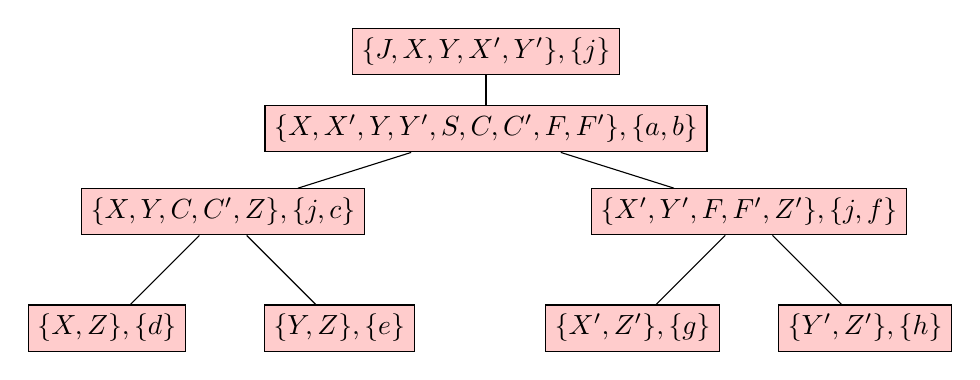
\begin{tikzpicture}%[level/.style={sibling distance=40mm,level distance=15mm}]
[level 1/.style={scale=1.0, fill=red,
    level distance=28pt, sibling distance=150pt},
    level 2/.style={ scale=1.0,
    level distance=30pt, sibling distance=190pt},
    level 3/.style={ scale=0.7,
    level distance=60pt, sibling distance=120pt}]
    level 4/.style={ scale=0.7,
    level distance=60pt, sibling distance=120pt}]  
    \tikzstyle{every node}=[rectangle,draw,fill=red!20]
    \node [rectangle,draw,fill=red!20]{$\{J,X,Y,X',Y'\},\{j\}$}
        child { 
            	node[rectangle,draw,fill=red!20] {$\{X,X',Y,Y',S,C,C',F,F'\},\{a,b\}$}
        		child { 
        			node[rectangle,draw,fill=red!20] {$\{X,Y,C,C',Z\},\{j,c\}$}
			child{
				node[rectangle,draw,fill=red!20] {$\{X,Z\},\{d\}$}
			}
			child{
				node[rectangle,draw,fill=red!20] {$\{Y,Z\},\{e\}$}
			}
		}
		child{
      			node[rectangle,draw,fill=red!20] {$\{X',Y',F,F',Z'\},\{j,f\}$}
			child{
				node[rectangle,draw,fill=red!20] {$\{X',Z'\},\{g\}$}
			}
			child{
				node[rectangle,draw,fill=red!20] {$\{Y',Z'\},\{h\}$}
			}
		}
	}
    ;
\end{tikzpicture}
\end{center}
\caption{A sample of hyper tree decomposition of the query $Q'$ defined \eqref{q'}}
\label{fig:hypertree}
\end{figure}
A hypertree of query $Q'$ is  shown in Figure~\ref{fig:hypertree}. The hypertree width is 2 in this case. 
\subsection{Number of different nodes or trees is polynomial}
In \cite{2} they defined AGCA(which is stands for AGgregation CAlculus). For each query they defined a delta for it which is a query again. They introduce \emph{delta queries} for incrementally view maintenance. Let $u$ denote a change(un insertion or deletion) to database $D$. Applying $u$ to the database $D$ is shown by $D+u$. Here ``+'' denotes a function which applies $u$ into $D$. A delta query $\Delta Q$ expresses the change to the result of query $Q$ as database $D$ is updated to $D+u$. We also used theirs notation to for $\Delta_{u}(Q)$ or $\Delta_{\pm R(\vec{t})}Q$ to denote the delta-query for such an update.

In this section we are suppose that a hypretree decomposition for a query is given. Applying $\Delta$ to it with any possible change produces a new tree. What we are interested is how many nodes this process will introduce. 

\begin{theorem}
\label{thm:1}
The number of all nodes in all possible delta trees is polynomial in terms of the number of relation, if hypertree width is fixed(independent of the number of relations). 
\end{theorem}
\begin{proof}
Let $k$ to be the hypertree width of the given hypertree decomposition of query $Q$ ($HT_{Q}$). Here we consider the case when $k$ is constant (we have an upper bound for it).
%When we apply the $\Delta$-operator to a join tree its nodes change also the structure. Here we prove that the number of all nodes in all different trees that emerge from all different sequence of applying the $\Delta$-operator is polynomial in term of $n$ for a fixed $k$.

Each node of $HT_{Q}$ contains at most $k$ different relations joining together. In the other words, without loss of generality each node is in form $R_{i_{1}}\Join\cdots\Join R_{i_{m}}$ which $m\leq k$. Lets fix one particular node as $l$ with $m$ relations and the set of its indices is $I$. If we apply $\Delta_{\pm R_{i_{p}}}$ when $i_{p}\not\in I$ this node will be $\emptyset$. For the other case we will have node $R_{i_{1}}\Join\cdots R_{i_{p-1}}\Join R_{i_{p+1}}\cdots R_{i_{m}}$, in the other words relation $R_{i_{p}}$ was deleted from node $l$.\\
Thus, for counting the number of all nodes in all $HT_{Q}$ for all sequences of applying $\Delta_{\pm R_{i}}$, we should count all nodes which contain $1,2,\cdots,k$ different relations. This number is 
\begin{equation}
\sum_{i=1}^{k}{\binom{n}{i}}<(n+1)^{k}
\end{equation}
which is polynomial for a fixed $k$. 
%The nodes of $HT_{Q}$ are all in form of $R_{i_{1}}\bowtie\cdots\bowtie R_{i_{m}}$ which $m\leq k$, $m$ relations join together. Lets fix one particular node as $l$ with $m$ relations and the set of its indices is $I$. If we apply $\Delta_{\pm R_{i_{p}}}$ when $i_{p}\not\in I$ this node is $\emptyset$. For the other case we will have node $R_{i_{1}}\bowtie\cdots R_{i_{p-1}}\bowtie R_{i_{p+1}}\cdots R_{i_{m}}$, in the other words relation $R_{i_{p}}$ was deleted from the join operation. Thus, for counting the number of all nodes in all $JT_{Q}$ for all sequences of applying $\Delta$-operator, we should count all nodes which contain $1,2,\cdots,k$ different relations. This number is 
%$\sum_{i=1}^{k}{\binom{n}{i}}<(n+1)^{k}$ which is polynomial for a fixed $k$. 
\end{proof}

There is another theorem like Theorem~\ref{thm:1} but for the structure of all possible trees.
\begin{theorem}
\label{thm:2}
The number of different structures of all these trees are polynomial for a constant hypertree width.
\end{theorem}
\begin{proof}
If $\Delta_{\pm R}$ applies to a join tree it won't change the nodes that do not contain relation $R$. Thus, without loss of generality we can assume that $R$ has appeared in all nodes  for the worst case(i.e. Figure~\ref{fig2}). \par

When we apply $\Delta_{\pm R}$ to a tree, each node splits into 3 different nodes($\Delta(R\Join S)=\Delta(R)\Join S+R\Join\Delta(S)+\Delta(R)\Join\Delta(S)$) \cite{2}. In the worst case, for each node at most 3 new nodes is created, thus, the number of nodes remains linear in term of the number of original nodes in the hypertree. \par
We can say the same thing for the cost of evaluation of the hypertrees. 
If we consider each $+,\Join$ as one operation, evaluation of $\Delta(R\Join S)$ needs at most 5 operations. Thus, the cost of evaluation of all $\Delta$ trees is $O(n)\times(\text{Cost of join operator})$.
\begin{figure}[htbp]
\begin{center}
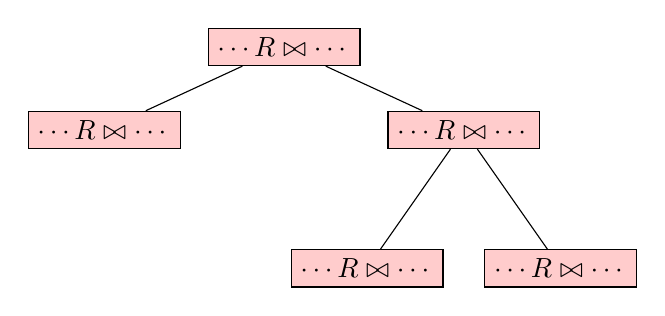
\begin{tikzpicture}%[level/.style={sibling distance=40mm,level distance=15mm}]
[
    %
    level 1/.style={rectangle, draw,scale=1.0, fill=red,
    level distance=30pt, sibling distance=130pt},
    level 2/.style={rectangle, draw, scale=1.0,
    level distance=50pt, sibling distance=70pt}]
    \tikzstyle{every node}=[rectangle,draw,fill=red!20]
    \node {$\cdots R\bowtie \cdots$}
        child { 
            node {$\cdots R\bowtie \cdots$}
        }
        child { 
        		node {$\cdots R\bowtie \cdots$}
		child{
       		node {$\cdots R\bowtie \cdots$}
		}
		child{
       		node {$\cdots R\bowtie \cdots$}
		}		
	}
    ;
\end{tikzpicture}
\end{center}
\caption{A worst case tree for Theorem~\ref{thm:2}}
\label{fig2}
\end{figure}
\end{proof}
\subsection{Hypertree Decomposition}
Gottlob et al. have shown that for each Hypertree there exists a join tree with the same tree structure(Lemma 4.6)\cite{1}. Thus, we have these results for join trees too. The advantage of hyperrtrees over the join trees is that the hypertree width is always less than or equal to the tree width. Also, acyclic queries may have unbounded tree width\cite{1}.\\\par

We can compute the hypertree decomposition in several ways. Each definitions of dual graph, hyper graph and primal graph will result into a decomposition.
\par
If we want to find a hypertree decomposition using the dual graph, for each node we need to select some relations for joining together. The act of selecting the relations is contracting some nodes in the corresponding dual graph. \\ \par
For hypergraph model we can do the same process, but here we select a set of vertices which are the variables and contract them together.
\section{Algorithms}
In this section we present an algorithm for computing  $\Delta$ of a hypertree of a query with respect to a relation.
Suppose we want to compute $\Delta_{\pm R}{HT_{Q}}$. As we had in Theorem~\ref{thm:2} for the worst case we can assume that every node contains relation $R$ (i.e. \ref{fig3}) or has a variable which represents a subquery that contains $R$.
\begin{figure}[htbp]
\begin{center}
\usetikzlibrary{fit}
\begin{tikzpicture}%[level/.style={sibling distance=40mm,level distance=15mm}]
[
    %
    level 1/.style={scale=1.0, fill=red,
    level distance=30pt, sibling distance=150pt},
    level 2/.style={ scale=1.0,
    level distance=30pt, sibling distance=70pt},
    level 3/.style={ scale=0.7,
    level distance=60pt, sibling distance=120pt}]
    
%    \tikzstyle{every node}=[rectangle,draw,fill=red!20]
    \node [rectangle,draw,fill=red!20]{$\cdots R\Join \cdots$}
        child { 
            node[rectangle,draw,fill=red!20] {$\cdots R\Join \cdots$}
        }
        child { 
        		node[rectangle,draw,fill=red!20] {$\cdots R\Join \cdots$}
		child{
       		node[rectangle,draw,fill=red!20] {$\cdots R\Join \cdots$}
		}
		child{
       		node[rectangle,draw,fill=red!20] {$\cdots R\Join \cdots$}
		child{
			node(b) [rectangle,draw,fill=red!20]{$\cdots R\Join \cdots$}
		}
%		child{
%			node{$\cdots$}
%		}
		child{
			node (a) [rectangle,draw,fill=red!20]{$\cdots R\Join \cdots$}
		}
		}		
	}
    ;
    \draw[dotted] (a) -- (b);
    \node(ff)[draw=blue,inner sep=0pt,thick,ellipse,fit=(a) (b)] {};
    \node[below=3mm of ff ] {j elements};
\end{tikzpicture}
\end{center}
\caption{Computing the $\Delta_{\pm R}$}
\label{fig3}
\end{figure}

\begin{algorithm}[H]
\caption{Computing $\Delta_{\pm R}(v)$} 
\label{alg1}
\textbf{Input:} node $v$ as the root of $HT_{Q}$ and relation $R$ as the $\Delta$ variable.\\
\textbf{Output:} Calculus expression for $\Delta_{R}$ for node $v$
\begin{algorithmic}[1]
\STATE $J\gets $ all relations and variables in $v$
\FORALL{Child $i$ of node $v$}
\IF{ $T_{i}$ has any node labeled by $R$ or a $t$ for which $R\in t$}
\STATE Computes the $\Delta_{R}$ of $i$ recursively and store it in $\Delta[i]$ if it is not already computed.
\STATE add $i$ to $J$
\ENDIF
\ENDFOR
%\STATE $Exp\gets\emptyset$
\STATE $value\gets ComputeChain(J)$
\RETURN $value.expr$
\end{algorithmic}
\end{algorithm}

\begin{algorithm}[H]
\caption{ComputeChain$(J)$} 
\label{alg2}
\textbf{Input:} A set of sibling nodes of $HT_{Q}$ as $J$ and relation $R$ as the $\Delta$ variable.\\
\textbf{Output:} Calculus expression for $\Delta_{R}$ for input nodes\\
\begin{algorithmic}[1]
\IF{$|J|=1$}
\STATE $expr\gets \Delta_{R}(J_{1})$ \COMMENT{$J_{1}$ is the first element of $J$}
\STATE $join\gets J_{1}$
\ELSE
\STATE $rest\gets ComputeChain(J\setminus J_{1})$
\STATE $join\gets J_{1}\Join rest.join$
\STATE $expr\gets rest.expr\Join \Delta(J_{1})+\Delta(J_{1})\Join rest.join+J_{1}\Join rest.expr$
\ENDIF
\RETURN $(exp,join)$
\end{algorithmic}
\end{algorithm}
Algorithm~\ref{alg1} computes the $\Delta_{\pm R}$ of any hypertree. At each node $v$ we check if the subtree rooted at $v$ contains any node with label $R$ or any variables as a subquery which the subquery contains $R$. In either of these two cases we compute the $\Delta_{\pm R}$ of the subtree, otherwise its $\Delta_{\pm R}$ is zero. \\
The computation is straightforward. For computing the delta of each node $v$, we first compute the delta of its children recursively  and then $v$ itself. This is done in Algorithm~\ref{alg1}. 
\par
The algorithm needs to compute the delta of each node just one time. If we want to compute the delta of a node with branching factor $k$ it needs $2^{k}-1$ different joint operation($\Join$) which is exponential in the worst case. But we can use a simple trick here. For the node we can first consider $\Delta_{\pm R}$ of $k-1$ children and store it somewhere then with this value we can merge the $k$th one. With Algorithm~\ref{alg2} we can compute the $\Delta_{\pm R}$ in $O(n)$.
%\section{Relation between hypertrees and parse trees}
%In this section we 


\section{Nested queries}

In this section we are going to talk about nested queries and how the algorithm for computing the delta queries will be applied to such queries. 

For example if we have the following query:

\begin{align}
\label{query:nest}
&\mbox{SELECT COUNT(*) }\\
&\mbox{FROM R}\nonumber\\
&\mbox{WHERE R.a}<\mbox{(SELECT sum(c) FROM S WHERE R.b=S.b)}\nonumber
\end{align}

Query \ref{query:nest} is a nested query because all of its records are influenced by the result offered by the inside query. When transforming the query into DBToaster Calculus we are going to have the following expression:
\begin{align}
\sum(R\cdot(R.a<\sum[(S.b=R.b)\cdot S.c]))
\end{align}
However this expression can be modified so that inequalities will appear only between variables, and therefore introduce an assignment operator ``$\gets$'':
\begin{align}
\label{form}\sum(R\cdot(t\gets\sum[(S.b=R.b)\cdot S.c])\cdot(R.a<t))
\end{align}

Considering the representation of a hyper graph, we can represent the connections between the variables of the previous example. In a hyper graph the vertices are the variables and the edges represent the relations between these vertices. Taking into account the previous example we have the following types:
\begin{enumerate}
\item relation R: which has the variables $a$ and $b$
\item the inequality $\theta$: which connects variable $a$ with variable $t$
\item the assignment $\gets$: which connects variable $t$ with variable $b$, because $t\gets q_{1}$ with bound variable $b$
\end{enumerate}
\begin{align}
\label{hyper}
\setlength{\unitlength}{1mm}
\begin{picture}(50,50)
\put(50,30){\line(-3,2){30}}
\put(20,50){\line(-1,-4){10}}
\put(10,10){\line(2,1){40}}
\qbezier(50,30)(10,10)(20,50)
\put(50,30){$a$}
\put(20,50){$t$}
\put(8,8){$b$}
\put(30,15){$R$}
\put(37,40){$\theta$}
\put(10,30){$\gets$}
\put(24,27){\mbox{cut line}}
\end{picture}
\end{align}

Figure \ref{hyper} represents a hype graph representation of the connections between the variables that appear in the formulae \ref{form}. We make a cut through the hyper graph along the variables $a$ and $t$. After this cut we can construct a tree which resembles very much a parse tree.

\begin{figure}[htbp]
\begin{center}
\usetikzlibrary{fit}
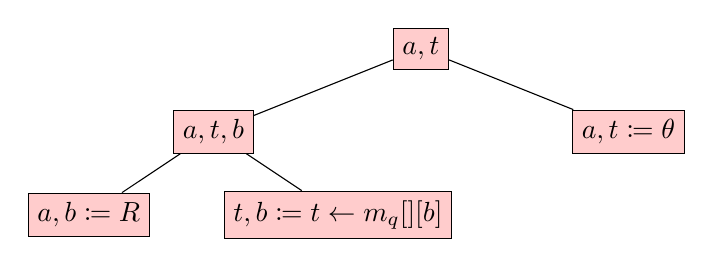
\begin{tikzpicture}%[level/.style={sibling distance=40mm,level distance=15mm}]
[
    %
    level 1/.style={scale=1.0, fill=red,
    level distance=30pt, sibling distance=150pt},
    level 2/.style={ scale=1.0,
    level distance=30pt, sibling distance=90pt},
    level 3/.style={ scale=0.7,
    level distance=60pt, sibling distance=120pt}] 
    \tikzstyle{every node}=[rectangle,draw,fill=red!20]
    \node [rectangle,draw,fill=red!20]{$a,t$}
        child { 
            	node[rectangle,draw,fill=red!20] {$a,t,b$}
        		child { 
        			node[rectangle,draw,fill=red!20] {$a,b\coloneqq R$}
				}
				child{
      				node[rectangle,draw,fill=red!20] {$t,b\coloneqq t\gets m_q[][b]$}
				}
	}
	child {
	node[rectangle,draw,fill=red!20] {$a,t\coloneqq\theta$}
	}
    ;
\end{tikzpicture}
\end{center}
\caption{A decomposition of the query \ref{form}}
\label{figtree}
\end{figure}
As you can see the decomposition of the example query is a parse tree, which will have as leaves the connections between the variables of the query. When talking about variables $t$ and $b$, these variables participate in the assignment of the value of the subquery to the variable $t$. The result offered by the subquery will be influenced by the value of $b$ from relation $R$. Therefore we can substitute the subquery with a data structure which keeps the values for each different $b$: we substitute it with a map, which is a function defined on the domain of variable $b$ and which offers results for each value of $b: m_q[][b]\coloneqq\sum[(S.b=R.b)\cdot S.c]$.

The subquery can also be further down decomposed:
\begin{align}
\label{hyper1}
\setlength{\unitlength}{1mm}
\begin{picture}(50,50)
\put(40,20){\line(-3,2){30}}
\put(40,20){$b$}
\put(10,40){$c$}
\put(27,30){$S$}
\end{picture}
\end{align}
In the hyper graph \ref{hyper1} we have just a simple relation. However in a more general case the sub queries can be more complicated. Another method of obtaining a decomposition of a query is by using the dual graph of the hypertree. We know that a dual graph will be graph which has as vertices the relations and as edges the variables that make the connection between those relations. Going back to the example~\ref{query:nest}, we can represent that query as follows:

\begin{align}
\label{hyper3}
\setlength{\unitlength}{1mm}
\begin{picture}(50,50)
\put(50,30){\line(-3,2){30}}
\put(20,50){\line(-1,-4){10}}
\put(10,10){\line(2,1){40}}
\put(10,10){\line(5,0){14}}
\put(50,30){$R$}
\put(20,50){$\theta$}
\put(8,8){$\gets$}
\put(25,8){$S$}
\put(30,15){$b$}
\put(37,40){$a$}
\put(10,30){$t$}
\put(18,10){$b$}
\end{picture}
\end{align}

We have treated the inequality as a relation and therefore put it on the dual graph representation as a vertex, as well for the assignment operator. However the vertex representing the assignment operator is connected with relation $R$ and relation $S$ through the variable $b$. The variable $b$ from relation $R$ influences the result of the subquery, because of the $equal$ between relation $R$ and $S$: $R.b=S.b$.

Having this representation we can make cuts through relations and therefore we can obtain a tree decomposition of the query. Each node of the tree is represented by relations and the edges are the connections between relations that are mapped to different nodes.

Having this example and the extensions of hyper edges in section \ref{sec:generalization}, we can say that the ideas for performing the tree decomposition, even when having inequalities and assignments, will work in the general case. 

\begin{thebibliography}{9}
\bibitem{2} C. Koch, \emph{Incremental Query Evaluation in a Ring of Databases},  preprint (2011).
%\bibitem{3} O. Kennedy, Y. Ahmad, C. Koch. \emph{DBToaster: Agile views for a dynamic data management system}. In CIDR, 2011.
\bibitem{1} Georg Gottlob, Nicola Leone and Francesco Scarcello, \emph{Hypertree Decompositions and Tractable Queries} J. Comput. Syst. Sci., 2002.
\end{thebibliography}
\end{document}
